\documentclass[../main.tex]{subfiles}
\newcommand{\coset}[1]{\code{#1}+C}

\begin{document}

\subsection{Introduction}		
\begin{defn}
	A \textbf{\emph{linear code}} $C$ over $GF(q)$ is a subspace of $V(n,q)$. 
\end{defn}		
\textbf{Notation:} If linear code $C$ is a $k$-dimensional subspace of $V(n,q)$ with minimum distance $d$, $C$ is denoted by $[n,k]$-code or $[n,k,d]$-code depending on the context.\\

The \textbf{\emph{weight}} w($\code{x}$) of a vector $\code{x}$ in $V(n,q)$ is the number of non-zero entries of $\code{x}$.
\begin{lem}\label{lem_diswiegh}
	If $\code{x}$ and \code{y} $\in V(n,q)$ then 
	\[
		\dis{x}{y}=w(\code{x}-\code{y}).
	\]
\end{lem}
\begin{proof}
	$\code{x}-\code{y}$ will be non-zero exactly at those places where \code{x} and  \code{y} differ.
\end{proof}
\begin{thm}
	Let $C$ be a linear code and let $w(C)$ be the smallest of the non-zero weights. Then $d(C)=w(C).$ 
\end{thm} 
\begin{proof}
	Let \code{x} and \code{y} be codewords with distance $d(C)$. Then by Lemma \ref{lem_diswiegh},
	\[
		d(C)=w(\code{x}-\code{y}) \geq w(C)
	\]
	as $\code{x}-\code{y}\in C$. Let \code{z} be a codeword such that $w(\code{z})=w(C)$. Since $\code{0}\in C$, by Lemma \ref{lem_diswiegh} again,
	\[
		w(C)=w(\code{z}-\code{0})=\dis{z}{0}\geq d(C).
	\]
	Therefore, $d(C)=w(C)$.
\end{proof}
This theorem allows us to calculate $d(C)$ in $M$ iterations, which otherwise would have been $\binom{M}{2}=\frac{M(M-1)}{2}$, one of the reasons we focus on linear codes. One more reason being that every codeword can be expressed in terms of $k$ codewords, in the case of $[n,k]$-code, we don't have to list all the codewords.  	

\begin{defn}
	A $k\times n$ matrix whose rows form a basis of a linear $[n,k]$-code is called a \textbf{\emph{generator matrix}} of the code.
\end{defn}
\begin{defn}
	Two linear codes are said to be \textbf{\emph{equivalent}} if one can be obtained from another by combinations of operations of the types,\;
	\begin{enumerate}[label=(\roman*)]
	\itemsep-1mm
		\item permuations of the positions of the code.
		\item multiplication of the symbols of fixed position by a non-zero scalar.
	\end{enumerate}
\end{defn}

\begin{thm}\label{thm_lc_equimatrices}
	Two $k\times n$ matrices generate equivalent linear $[n,k]$-codes over $GF(q)$ if one can be obtained from other by a sequence of these operations.
	\begin{enumerate}[label=(\roman*)]
	\itemsep-1mm
		\item Permutations of the rows.
		\item Multiplication of a row by a non-zero scalar.
		\item Addition of the scalar multiple of one row to another.
		\item Permutations of the columns.
		\item Multiplication of any column by a non-zero scalar.
	\end{enumerate}
\end{thm}
\begin{proof}
	The first three operations are called \textbf{\emph{row operations}}, and they will preserve the linear independence of the row vectors and will replace one basis by another of the same code. Last two are called \textbf{\emph{column operations}}, they convert the basis into basis of a equivalent code. 
\end{proof}

\begin{thm}
	Let $G$ be a generator matrix of an $[n,k]$-code. Then by operations described in Theorem \ref{thm_lc_equimatrices}, $G$ can be converted into \textbf{\emph{standard form}}
	\[
		[I_k\;|\;A],
	\]
	where $I_k$ is the $k\times k$ identitiy matrix, and $A$ is a $k\times (n-k)$ matrix.
\end{thm}
\begin{proof}
	Let $G=[g_{ij}]$ and $\code{r}_1,\code{r}_2,\ldots,\code{r}_k$ and $\code{c}_1,\code{c}_2,\ldots,\code{c}_n$ be its rows and columns respectively, then the following scheme will convert it to standard form.\\
	Suppose $G$ has already been transformed to
	\[
		\begin{bmatrix}
			1 & \cdots & 0 & g_{1j} & \cdots & g_{1n}\\
			\vdots & \ddots & \vdots & \vdots & & \vdots\\
			0 & \cdots & 1 & g_{j-1,j} & \cdots &g_{j-1,n}\\
			0 & \cdots & 0 & g_{jj} & \cdots & g_{jn}\\
			\vdots &  & \vdots & \vdots &  & \vdots\\
			0 & \cdots & 0 & g_{kj} & \cdots & g_{kn}\\
		\end{bmatrix}
	\]
	where $j\in \{1,2,\ldots,k\}$.\\
	\begin{enumerate}
	\itemsep-1mm
		\item If $g_{jj}\neq 0$, proceed to next step. If $g_{ij}=0$, if for some $i>j$, $g_{ij}\neq 0$, replace $\code{r}_j$ with $\code{r}_i$. If not, replace $\code{c}_j$ with $\code{c}_p$, where $g_{jp}\neq 0$. (We could have sone the column step directly without looking for the row first, but we are trying that the matrix remains basis of the original code $C$, if possible.)
		\item Multiply $\code{r}_{j}$ with $g_{jj}^{-1}$, so that $g_{jj}$ becomes $1$.
		\item For each $i\in \{1,2,\ldots,k\}, i\neq j$, convert $\code{r}_i\rightarrow \code{r}_i-g_{ij}\code{r}_j$.
	\end{enumerate}
	Now after these steps, we have converted $\code{c}_j$ to the the required form. So repeating for all values of $j$ will give the standard form. 	 
\end{proof}
\textbf{Note:} \emph{Standard form} of a generator matrix is not unique, for instance we can interchange the columns of $A$ and still satisfy all the conditions. Also, the standard form will remain generator matrix of the original code $C$ iff we don't use the column operations. It is possible if and only if the first $k$ columns of generator matrix are \emph{linearly independent}. 

\subsection{Encoding with a linear code}

Let $C$ be an $[n,k]$-code over $GF(q)$ with generator matrix $G$. It can be used to communicate $q^k$ distinct messages. If the rows of $G$ are $\code{r}_1,\code{r}_2,\ldots,\code{r}_k$, then we \emph{encode} a message vector $\code{u}=u1u2\cdots u_k \in V(k,q)$ by a function that maps $V(k,q)\rightarrow k$-dimensional subspace of $V(n,q)$ (the code $C$).
\[
	\code{u}G = \displaystyle\sum_{i=1}^{k}u_i\code{r}_i
\] 
In particular, if $G=[I_k\;|\; A]$ (standard form, $A=[a_{ij}]$), then encoding is $$\code{x} = \code{u}G=x_1x_2\cdots x_k\cdots x_n,$$ where $x_i=u_i$, $1\leq i\leq k$ are \textbf{\emph{message digits}}, and 
\[
	x_{k+i}=\displaystyle\sum_{j=1}^{k}a_{ij}u_{j}\hspace{5mm} 1\leq i\leq n-k,	
\]
are the \textbf{\emph{check digits}}. The check digits represent \emph{redundancy} added to protect against noise.\\

\begin{figure}[h]
	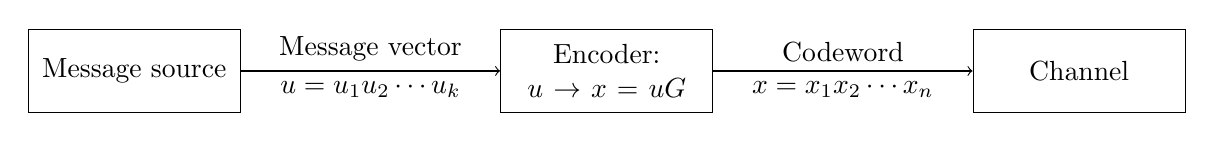
\begin{tikzpicture}[rect/.style={draw,align=center,text width=7em,minimum height=3em]}]
		\node[rect]      (l)                          {Message source};
		\node[rect]      (c)      [right of= l,node distance=6cm] 	{Encoder:\\ $\code{u}\rightarrow\code{x}=\code{u}G$ };
		\node[rect]      (r)       [right of= c,node distance=6cm] {Channel};
		
		\draw[->] (l.east)  -- (c.west) node[midway, above] {Message vector} node[midway, below] {$\code{u}=u_1u_2\cdots u_k$};
		\draw[->] (c.east) -- (r.west) node[midway, above] {Codeword} node[midway, below] {$\code{x}=x_1x_2\cdots x_n$};
	\end{tikzpicture}
	\centering
	\caption{Encoding a message vector.}
\end{figure}

\subsection{Decoding with a linear code}
Suppose the codeword sent is $\code{x}=x_1x_2\cdots x_n$ and the recieved vector is $\code{y}=y_1y_2\cdots y_n$. We define \textbf{\emph{error vector}} $\code{e}$ to be
\[
	\code{e}=\code{y}-\code{x}=e_1e_2\cdots e_n.
\]

\begin{defn}
	Suppose that $C$ is an $[n,k]$-code over and \code{a} is any vector in $V(n,q)$. Then set
	\[
		\code{a}+C=\{\code{a}+\code{x}\;|\; \code{x}\in C\}
	\]
	is called a \textbf{\emph{coset}} of $C$.
\end{defn}
\begin{lem}\label{lem_selfcontd_cosets}
	Suppose that $\code{x}+C$ is a coset of $C$ and $\code{b}\in \code{a}+C$. Then $\code{b}+C=\code{a}+C$.
\end{lem}
\begin{proof}
	Since $\code{b}\in \code{a}+C$, we have $\code{b}=\code{a}+\code{x}$ for some $\code{x}\in C$. Now if $\code{b}+\code{y}\in \code{b}+C$, then
	\[
		\textbf{b}+\textbf{y}=(\textbf{a}+\textbf{x})+\textbf{y}=\textbf{a}+(\textbf{x}+\textbf{y})\in \textbf{a}+C.
	\]
	Hence, $\code{b}+C\subseteq \code{a}+C$. Similarly, if $\code{a}+\code{z}\in \code{a}+C$, then
	\[
		\textbf{a}+\textbf{z}=(\textbf{b}-\textbf{x})+\textbf{z}=\textbf{b}+(\textbf{z}-\textbf{x})\in \textbf{b}+C.
	\]
	Hence, $\code{a}+C\subseteq \code{b}+C$. Therefore, $\code{b}+C=\code{a}+C$.
\end{proof}

\begin{thm}\label{thm_lagrange-subgroups}
	Suppose $C$ is an $[n,k]$-code over $GF(q)$. Then
	\begin{enumerate}[label=(\roman*)]
	\itemsep-1mm
		\item every vector of $V(n,q)$ is in some coset of $C$,
		\item every coset contains exactly $q^k$ vectors,
		\item two cosets are either disjoint or coincide.
	\end{enumerate}
\end{thm}
\begin{proof}
	\hfill
	\begin{enumerate}[label=(\roman*)]
	\itemsep-1mm
		\item If $\code{a}\in V(n,q)$, then $\code{a}=\code{a}+0\in \code{a}+C$
		\item It can be easily seen that the mapping $C\rightarrow \code{a}+C$ is one-one. Therefore, $|C|=|\code{a}+C|$.
		\item Suppose cosets $\coset{a}$ and $\coset{b}$ overlap and $\code{v}\in (\coset{a})\cap (\coset{b})$. Thus, for some $\code{x},\code{y}\in C$, 
		\begin{align*}
			& \code{v} = \code{a}+\code{x} = \code{b}+\code{y}\\
			\implies & \code{a} = \code{b}+\code{y}-\code{x}\\
			\implies & \code{a}\in \coset{b}\\
		\end{align*}
		Therefore, by Lemma \ref{lem_selfcontd_cosets}, $\coset{a}=\coset{b}$.   
	\end{enumerate}
\end{proof}

\begin{defn}
	The vector having minimum weight in a coset is called the \textbf{\emph{coset leader}}. (If there are more than one vectors with minimum weight then we choose anyone.)
\end{defn}

Theorem \ref{thm_lagrange-subgroups} implies:
\[
	V(n,q)=(\coset{0})\cup (\code{a}_1+C)\cup \cdots \cup (\code{a}_s+C)
\]
where $s=q^{n-k}-1$, and by Lemma \ref{lem_selfcontd_cosets}, we can take $\code{a}_i$ to be the coset leaders.\\
\begin{defn}
	A \textbf{\emph{standard array}} for an $[n,k]$-code $C$ is a $q^{n-k}\times q^k$ array of all the vectors of $V(n,q)$. First row will consist of code $C$ in any order except \code{0} which will be in in the first column. Following rows will be cosets with coset leaders being the first element of each row, remaining elements in each row will be sum of its coset leader with corresponding codeword in the same column. 
\end{defn}
For example, let $C$ be a binary $[4,2]$-code with generator matrix 
\[
	G = \begin{bmatrix}
		1 & 0 & 1 & 1\\
		0 & 1 & 0 & 1\\
	\end{bmatrix}
\]
then $C=\{0000,1011,0101,1110\}$.\\
The standard array of $C$ will be
\[
	\begin{matrix}
		\text{codewords}\rightarrow & 0000 & 1011 & 0101 & 1110\\
									& 1000 & 0011 & 1101 & 0110\\
									& 0100 & 1111 & 0001 & 1010\\
									& 0010 & 1001 & 0111 & 1100\\
									& \uparrow\\
									&\text{coset}\\
									&\text{leaders}
 	\end{matrix}
\]
\textbf{Decoding scheme using standard array:} When $\code{y}$ is recieved its position is found in array. Then the \emph{decoder} assumes that the error vector $\code{e}$ is the coset leader, and \code{y} is decoded as $\code{x}=\code{y}=\code{e}$ at the top of the column containing \code{y}. By choosing the minimum weight vector as the coset leader, we ensure that standard array decoding scheme is a nearest neighbour decoding scheme.

\begin{thm}
	Let $C$ be a binary $[n,k]$-code, and for $i\in \{1,2,\ldots,n\}$, let $\alpha_i$ denote the number of cosets leaders of weight $i$. Then \emph{probability} $P_{\text{corr}}(C)$ of correctly recognizing the codeword is given by
	\[
		P_{\text{corr}}(C) = \displaystyle\sum_{i=0}^{n}\alpha_ip^i(1-p)^{n-i}.
	\]
\end{thm}
\begin{proof}
	The probability of error code to be vector of weight $i$ is $p^i(1-p)^(n-i)$. Therefore, the result follows directly from the definition of decoding scheme.
\end{proof}
\textbf{Note:} If $d(C)=2t+1$ or $2t+2$, then $\alpha_i=\binom{n}{i}$ for $0\geq i\geq t$. In particular, if $C$ is a perfect code, in addition to the general result, $\alpha_i=0$ for $i>t$ also holds.

\begin{thm}
	Let $C$ be a binary $[n,k]$-code, and let $A_i$ denote the number of codewords of weight $i$. Then \emph{probability} $P_{\text{corr}}(C)$ of an error going undetected is given by
	\[
		P_{\text{undetec}}(C) = \displaystyle\sum_{i=1}^{n}A_ip^i(1-p)^{n-i}.
	\]
\end{thm}
\begin{proof}
	The error will only go undetected if and only if $\code{y}-\code{x}$ is a non-zero codeword, where \code{y} and \code{x} are received and sent vectors respectively. The probability of $\code{y}-\code{x} = \code{z}\in C$ is $p^{w(\code{z})}(1-p)^{n-w(\code{z})}$, thus summing over non-zero \code{z} gives the result. 
\end{proof}

\begin{defn}
	For a linear $[n,k]$-code $C$, \textbf{\emph{rate}} is defined as the ratio of number of message symbols to the total number of symbols sent, i.e. $R(C)=\dfrac{k}{n}$.
\end{defn}
Good code generally will have high rate.
\begin{defn}
	The \textbf{\emph{capacity}} $\mathscr{C}(p)$ of a binary symmetric channel with symbol error probability $p$ is
	\[
		\mathscr{C}(p) = 1 + p\log_2p + (1-p)\log_2(1-p).
	\] 
\end{defn}

\begin{thm}{\textbf{Shannon's Theorem}}
	Suppose a channel is binary symmetric with symbol error probability $p$. Let $R\in \mathbb{R}$ satisfying $R<\mathscr{C}(p)$. Then for all $\epsilon > 0$, there exists, for some large n, an $[n,k]$-code $C$ of rate $\dfrac{k}{n} \geq R$ such that $P_{\text{err}}(C)<\epsilon$. (where $P_{\text{err}}(C) = 1-P_{\text{corr}}(C)$)
\end{thm}
%\begin{proof}
%\end{proof}


\end{document}
